\documentclass[a4paper,10pt]{article}
\usepackage[utf8]{inputenc}
\usepackage{graphicx}
\usepackage{multirow}

%opening
\title{Sana Clinician Guide: Procedure Implementation}
\author{}

\begin{document}

\maketitle

\begin{abstract}

\end{abstract}

\section{Clinician User Guide: Procedures}
Targeted at a clinician who does not need to manage the information system. The 
guide will walk through the transfer of a paper-based medical questionaire into 
a format usable on a Sana mobile client. 

\subsection{Overview}
The implementation of a new \textbf{Procedure} is performed using an XML scheme 
which describes the instructions to execute, context for the data collected, and
logic which guides the mobile client user through the execution process. The 
\textbf{Procedure} document itself consists of a series of opening and closing
XML tags beginning with a \textbf{Procedure} and followed by at least one
\textbf{Page} which will contain at least one \texftbf{Element}. For example,
the following displays a single page and asks for text input.

\begin{verbatim}
<Procedure title="Simple Text Collection" author="Sana">
   <Page> 
     <Element type="ENTRY"
              id="1"
              concept="TEXT"
              question="Enter text" 
              answer=""/>
   </Page>
</Procedure>
\end{verbatim}

Following sections provide additional information on creating more complex
documents and the specification for the XML format.

\section{Procedure XML Specification} 
The following terms are the XML node tags and atttributes used when implementing
a \textbf{Procedure} as an XML formatted document. Attributes which are optional
are noted as such. Please see the \textbf{Development Guide} for advanced and 
beta features.

\subsection{Procedure}
\begin{description}
 \item [\textless Procedure\textgreater] Marks the beginning of procedure.
  \begin{description}
   \item[title] A descriptive name.
   \item[author] Who wrote the document.
   \item[uuid] (Optional)The id of the document.
   \item[version] (Optional)Distinguishes different versions of a protocol.
  \end{description}
\end{description}

\subsection{Page}
A \textbf{Page} groups one or more \textbf{Element} objects along with optional
conditional logic. On the mobile client, all \textbf{Element} objects will be
displayed as a single screen. The inclusion of conditional logic will require
that the conditional evaluates to \textbf{True} for the textbf{Page} to be 
visible.

\begin{description}
 \item [\textless Page\textgreater] Marks a set of one or more instructions 
 which are viewed collectively on a single page.
\end{description}

\subsection{Conditional Logic} 
The conditional logic available in the Sana \textbf{Procedure} mark up allows
for the introduction of branching logic as required by many decison trees. When
required, it must be included as the first child node for a \textbf{Page} within
the XML. Conditional statements that evaluate to \textbf{False} will prevent
the \textbf{Page} from being visible, or executed.

\begin{description}
 \item[\textless ShowIf\textgreater] The entry point for branching logic which 
 must logically evaluate to true for a Page to be displayed.
 \item[\textless Criteria\textgreater] An expression which will yield a logical 
 truth value when evaluated.
  \begin{description}
   \item[id] The id of the node to be used for comparison.
   \item[type] The type of comparison operator.
   \item[value] A value to compare against.
  \end{description}  
 \item[\textless and\textgreater] Logical conjunction between two or more 
 \textbf{Criteria}.
 \item[\textless or\textgreater] Logical disjunction between two or more 
 \textbf{Criteria}.
 \item[\textless not\textgreater] Logical negation of the result of a simple or 
 compound \textbf{Criteria}.
\end{description}

Please the section on \textbf{Predicate Logic} for use.

\subsection{Element}
The elements are the individual instructions which prompt the end user for input
or can be used to display information.

\begin{description} 
 \item [\textless Element\textgreater] A single \textbf{Instruction} node.
  \begin{description}
   \item[id] A unique identifier within the \textbf{Procedure}. The value is an
   arbitrary string but should limited to alphanumeric characters with no
   whitespace. 
   \item[type] A classification of the visual element to use.
   \item[concept] A term which provides context for the instruction.
   \item[question] The id of the document.
   \item[answer] A default value for the collected data.
   \item[choices] A  comma separated list of one or more options to choose from.
   Required for SELECT, RADIO, MULTI\_SELECT.
  \end{description}  
\end{description}

\section{Input Type Specification}
The following list gives a brief description of the elements available within a
\textbf{Procedure}. Additional details, screenshots, and sample mark-up for each
are provided. The value for the \textbf{type} attribute must be one
of the element types defined by the Sana application. The core element types 
are:

\begin{itemize}
 \item ENTRY
 \item SELECT
 \item MULTI\_SELECT
 \item RADIO
 \item GPS
 \item SOUND
 \item PICTURE 
\end{itemize}

\subsubsection{ENTRY} Presents a simple text box and collects text entered 
through the device keyboard.

\noindent\begin{tabular}{ p{3.5cm}  p{7.5cm} }
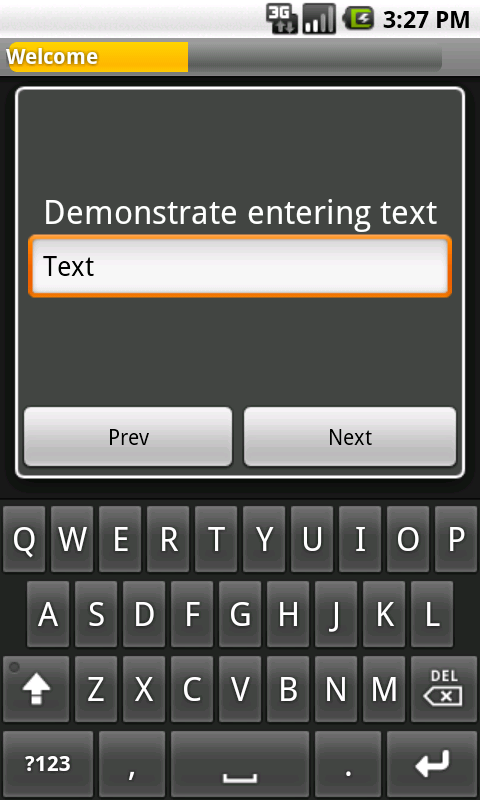
\includegraphics[scale=0.2,keepaspectratio=true]{client_entry_value.png}
& \begin{verbatim}<Element id="entry"
  type="ENTRY" 
  concept="TEXT"
  question="Entry Text"  
  answer=""/>\end{verbatim}
\end{tabular}

\subsubsection{SELECT} Presents a dropdown box and collects a single-item from a
list.

\noindent\begin{tabular}{ p{3.5cm}  p{7.5cm} }
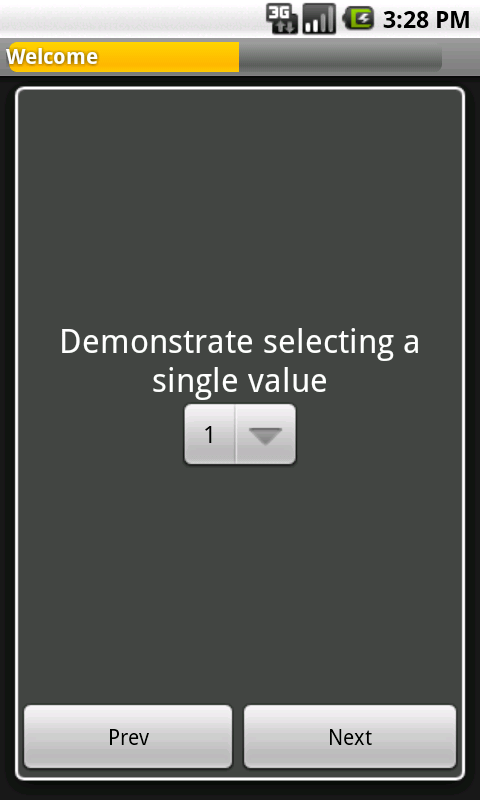
\includegraphics[scale=0.2,keepaspectratio=true]{client_select.png}
& \begin{verbatim}<Element id="entry"
  type="SELECT"
  concept="TEXT"
  question="Select a single value" 
  choices="1,2,3,4"
  answer=""/>\end{verbatim}
\end{tabular}


\subsubsection{MULTI\_SELECT} Collects one or more items from a list as a set of 
checkboxes.

\noindent\begin{tabular}{ p{3.5cm}  p{7.5cm} }
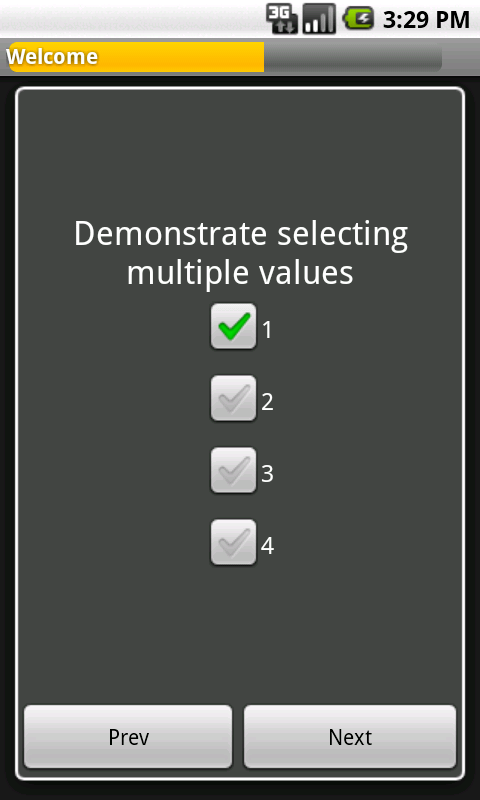
\includegraphics[scale=0.2,keepaspectratio=true]{client_multi_select.png}
& \begin{verbatim}
<Element id="multiSelect"
  type="MULTI_SELECT"  
  concept="TEXT"  
  question="Select one or more values"  
  choices="1,2,3,4"
  answer=""/>\end{verbatim}
\end{tabular}

\subsubsection{RADIO} Collects a single-item from a list as a set of radio
buttons.

\noindent\begin{tabular}{ p{3.5cm}  p{7.5cm} }
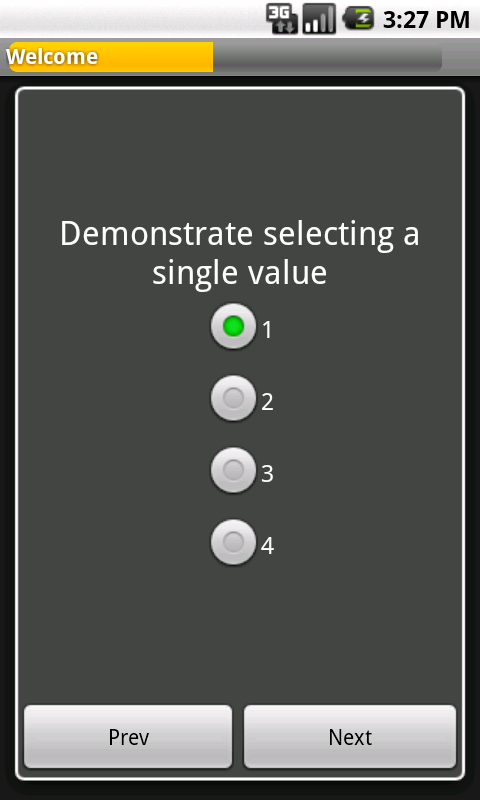
\includegraphics[scale=0.2,keepaspectratio=true]{client_radio.png}
& \begin{verbatim}
<Element id="radio"
    type="RADIO"  
    concept="TEXT"  
    question="Select a single value"  
    choices="1,2,3,4"
    answer="1"/>\end{verbatim}
\end{tabular}

\subsubsection{GPS} Collects coordinates through the device.

\noindent\begin{tabular}{ p{3.5cm}  p{7.5cm} }
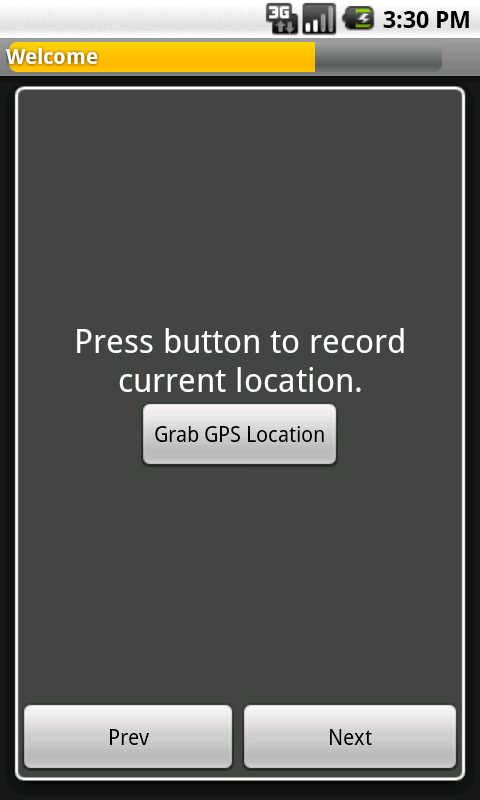
\includegraphics[scale=0.2,keepaspectratio=true]{client_gps.png}
& \begin{verbatim}
<Element id="gps"
    type="GPS"  
    concept="LOCATION"  
    question="Record the location."  
    answer=""/>\end{verbatim}
\end{tabular}

\subsubsection{SOUND} Collects audio using the device microphone.

\noindent\begin{tabular}{ p{3.5cm}  p{7.5cm} }
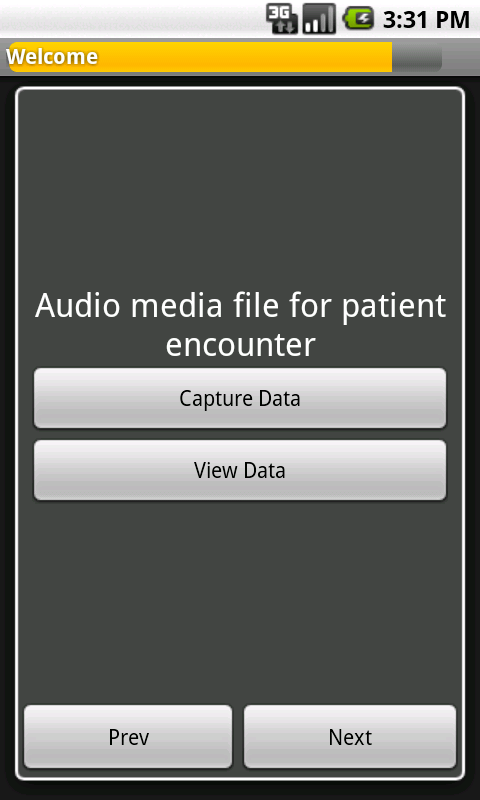
\includegraphics[scale=0.2,keepaspectratio=true]{client_audio.png}
& \begin{verbatim}
<Element id="sound"
    type="SOUND"  
    concept="AUDIO"  
    question="Record some audio"  
    answer=""/>\end{verbatim}
\end{tabular}

\subsubsection{PICTURE} Collects one or more images using the devices camera. 

\noindent\begin{tabular}{ p{3.5cm}  p{7.5cm} }
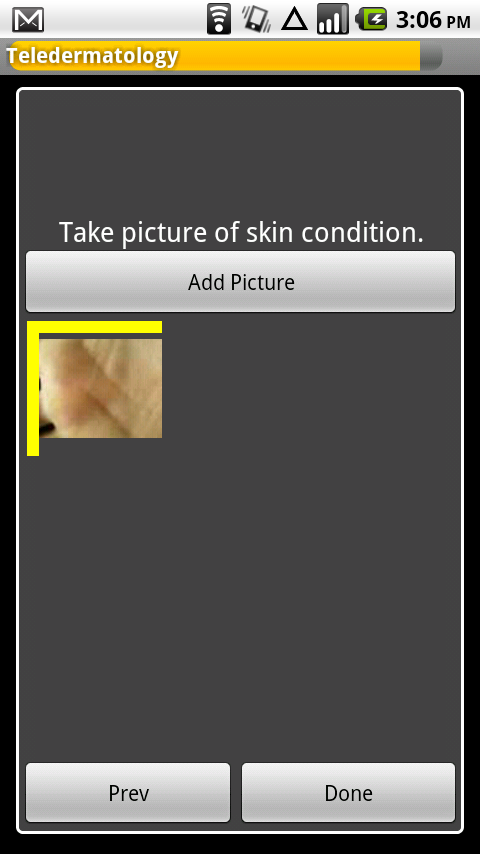
\includegraphics[scale=0.2,keepaspectratio=true]{client_picture.png}
& \begin{verbatim}
<Element id="image"
    type="PICTURE"  
    concept="IMAGE"  
    question="Take a picture."
    answer=""/>\end{verbatim}
\end{tabular}

\subsection{Concepts-providing context}
Sana requires each instruction to have a a concept attribute which provides the
context for the data collection. Prior to execution,all concepts used within a
ing a new \textbf{Procedure} must be defined on the server where the data will
ultimately be stored. If you would like to introduce new terms, please consult
with your system administrator regarding local policies for doing so.
Note: See the Advanced Content Creation Guide for more details and assitance. 

\subsection{Medical Decision Trees, or How to implement Branching Logic}
This section describes how to implement branching logic in Sana Procedure XML
douments. 

\subsubsection{Predicate logic}
Branching logic is included as simple or compound if/then conditional statements
as a way of choosing to display or not display certain questions. The condition
is evaluated using one of set of pre-defined compariison operators and data 
collected previously during the encounter and enforced at the Page level and
applies to all elements in the page.
 
\begin{verbatim}
  <Page>
    <ShowIf>
      <Criteria type="EQUALS" id="1" value="Yes"/>
    <ShowIf>
    ... one or more <Element> nodes ...
  </Page>
\end{verbatim}

\subsubsection{Criteria, Comparison operators.}
Comparison operators are a more powerful way of using if/then logic. Sana
supports three comparison operators-equals, less than, and greater than-each of
which will return a logical truth value. The \textbf{id} attribute must 
reference an \textbf{Element} with an \textbf{id} attribute having the same
value within the \textbf{Procedure}. 

\begin{verbatim}
    <Criteria type="EQUALS" id="1" value="Yes"/>
    <Criteria type="LESS" id="1" value="1"/>
    <Criteria type="GREATER" id="1" value="1"/>
\end{verbatim} 

Evaluation returns a logical truth as by comparing the \textbf{value} attribute
of the referenced element to the \textbf{value} attribute of the 
\textbf{Criteria}. The examples above would be evaluated as:

\begin{verbatim}
    Element(id=1).value = "Yes"
    Element(id=1).value < 1
    Element(id=1).value > 1
\end{verbatim} 


\subparagraph{Equals} The comparison value may be any alphanumeric string.
\begin{verbatim}
    <ShowIf>
      <Criteria type="EQUALS" id="1" value="Yes"/>
    <ShowIf>
\end{verbatim}

\subparagraph{Less Than} The comparison value must be numeric.
\begin{verbatim}
    <ShowIf>
      <Criteria type="LESS" id="1" value="1"/>
    <ShowIf>
\end{verbatim}

\subparagraph{Greater Than} The comparison value must be numeric.
\begin{verbatim}
    <ShowIf>
      <Criteria type="GREATER" id="1" value="1"/>
    <ShowIf>
\end{verbatim}

\subsubsection{Boolean Operators - and, or, not.}
Sana includes boolean conjunction, disjunction, and negation operators for
constructing more complex branching logic.

\subparagraph{Conjunction} Logical \textbf{and} which evaluates to \textbf{True}
if and only if all child statements are \textbf{True}.
\begin{verbatim}
    <ShowIf>
      <and>
        <Criteria type="EQUALS" id="1" value="Yes"/>
        <Criteria type="EQUALS" id="2" value="No"/>
      </and>
    <ShowIf>
\end{verbatim}

\subparagraph{Disjunction} Logical \textbf{or} which evaluates to \textbf{True}
at least one child statement is \textbf{True}.
\begin{verbatim}
    <ShowIf>
      <or>
        <Criteria type="EQUALS" id="1" value="Yes"/>
        <Criteria type="EQUALS" id="2" value="No"/>
      </or>
    <ShowIf>
\end{verbatim}

\subparagraph{Negation} Logical \textbf{and} which evaluates to \textbf{True}
if  child statement is \textbf{False}.
\begin{verbatim}
    <ShowIf>
      <not>
        <Criteria type="EQUALS" id="1" value="Yes"/>
      </not>
    <ShowIf>
\end{verbatim}

\subsubsection{Compound Predicates}
Predicate statements can include nesting a number of statements in order to
significantly more complex logic. The following conditional is provided to
give some idea of the complexity that can be achieved but is by no means the
limit of what can be constructed. 

\begin{verbatim}
    <ShowIf>
      <and>
        <not>
          <Criteria .../>
        </not>
        <Criteria .../>
        <or>
          <Criteria .../>
          <Criteria .../>
        </or>
        ...
      </and>
    </ShowIf>
\end{verbatim}

\subsection{Note about Patient Registration}
Patient registration information is collected and, or, verified automatically at
the beginning of each encounter by automatically appending a series of 
registration questions to the front of the document. The following list
details the information automatically collected.

\begin{itemize}
 \item Identifier
 \item Given Name
 \item Family Name
 \item Date of Birth
 \item Gender
\end{itemize}

\subsection{Putting it all together}
Based on the information above, a significant number of decision trees can be 
tranlated into XML docuemnts. This section presents a simple decision tree and
walks through implementing as an XML procedure.

\noindent\begin{figure}[h]
 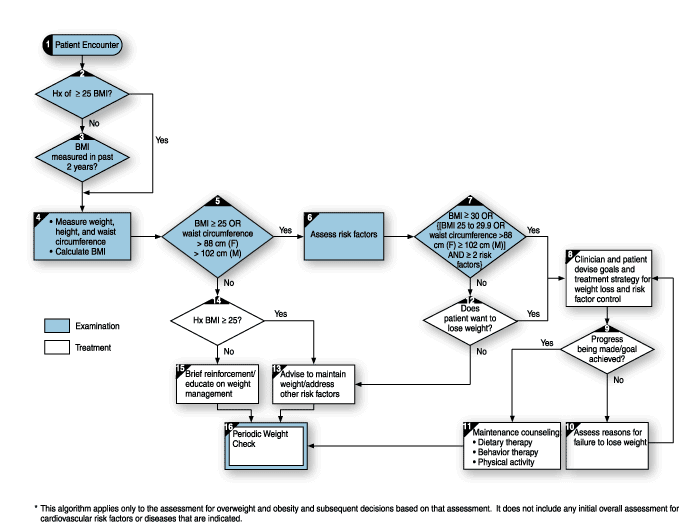
\includegraphics[scale=0.6,keepaspectratio=true]{Assessment_and_treatment_algorithm_for_overweight_and_obesity.png}
 % Assessment_and_treatment_algorithm_for_overweight_and_obesity.png: 682x525 pixel, 96dpi, 18.04x13.89 cm, bb=0 0 511 394
 \caption{Assessment and treatment algorithm for overweight and obesity}
\end{figure}

\begin{verbatim}
<Procedure title="Obesity Assessment" 
  author="National Heart, Lung, and Blood Institute">
  <Page>
    <Element id="1"
       type="RADIO" 
       concept="HX BMI RISK"
       question="History of BMI >= 25"
       choices="Yes,No"  
       answer=""/>
  </Page>
  <Page>
    <ShowIf>
      <Criteria id="1" type="EQUALS" value="Yes"/>
    </ShowIf>
    <Element id="2"
       type="RADIO" 
       concept="TWO YEAR HX BMI"
       question="BMI Measured in Past 2 Years"
       choices="Yes,No"  
       answer=""/>
  </Page>
  ...etc
\end{verbatim}

TODO: PROBABLY WANT TO USE A DIFFERENT QUESTIONNAIRE

\subsection{Using your new Procedure to collect data.}
New procedures require the Sana mobile client be installed on an Android based
mobile phone and that a copy of your new Procedure is available on the device.
If you're unsure of how to install or use the mobile client, see the 
Client User Guide. Getting a copy of the Procedure onto the phone can be done 
using one of two methods.

\begin{itemize}
 \item Compiling the Procedure into the application
 \item Downloading the Procedure onto phone's SDcard.
\end{itemize}
Unless you are a developer, copying the new procedure file to the phone SDcard
is the recommended method. 

\subsubsection{Downloading onto the SDcard}
Downloading the Procedure to the phone requires that it first be made available
on a webserver. Please consult your system adminstrator if unsure how/where to
upload the document to the web or the \textbf{SysAdmin} guide on how to set up a
Procedure repository. Once uploaded, the Procedure can be fetched from a mobile
client using the following steps.

\begin{itemize}
 \item Browse to the location on your phone.
      {IMAGE: Same webpage on a phone}
 \item Select the Procedure you want to Download.
  {IMAGE: Select a form --highlight it}
 \item Download the form to the following directory on your phone: \\ 
    \textbf{/mnt/sdcard/media/sana/resource/procedure} \\
  Note: You may need to use the phone filebrowser if unable to specify the
  destination directory.
\end{itemize}

\subsubsection{Loading the form into Sana}
Once downloaded and available in the correct directory, the Procedure is 
available to load into Sana using the following steps.

\begin{itemize}
 \item From the Sana app splash page, press \textbf{Menu} and then select
 \textbf{Settings}.
 \item Select \textbf{Sana Resources} 
 \item Select \textbf{Manage Procedures} 
 \item Procedures downloaded into the correct directory listed above will be 
 visible. They can be loaded individually by pressing on an item or have all
 available procedures loaded by pressing \textbf{Menu} and then
 \textbf{Load All}.
\end{itemize}

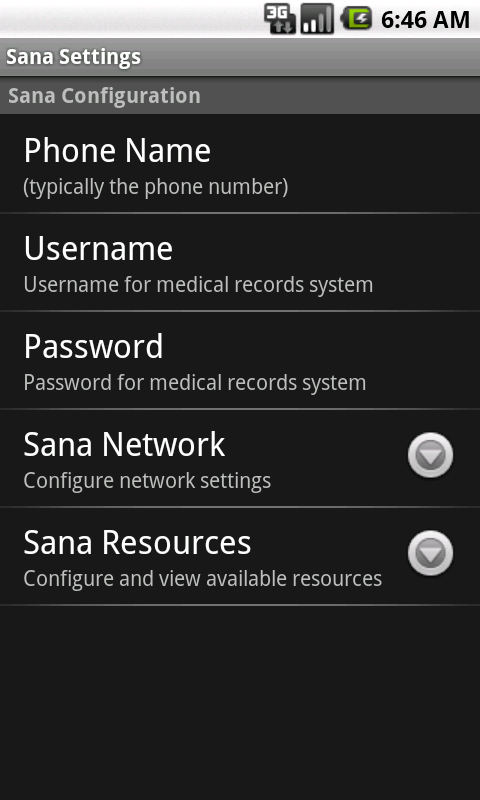
\includegraphics[scale=0.2,keepaspectratio=true]{client_settings.png}
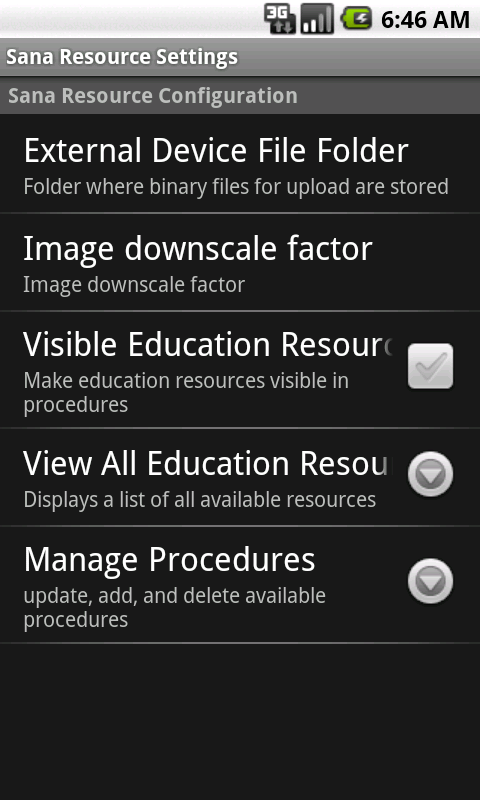
\includegraphics[scale=0.2,keepaspectratio=true]{client_settings_resources.png}
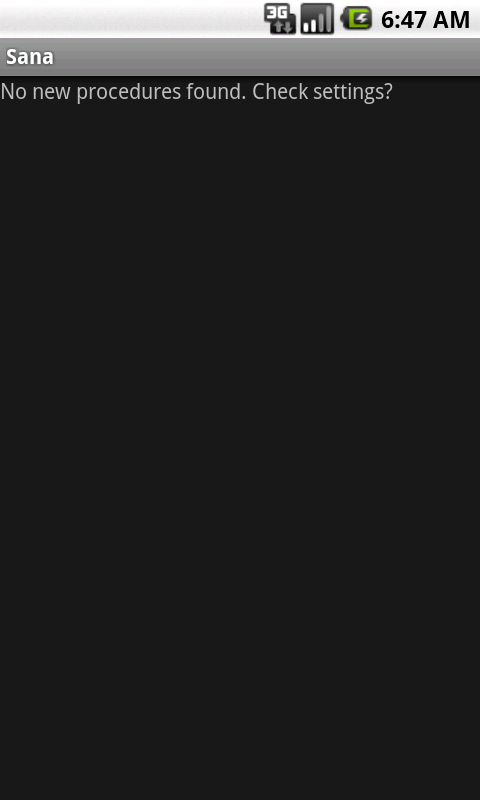
\includegraphics[scale=0.2,keepaspectratio=true]{client_settings_procedures_available.png}

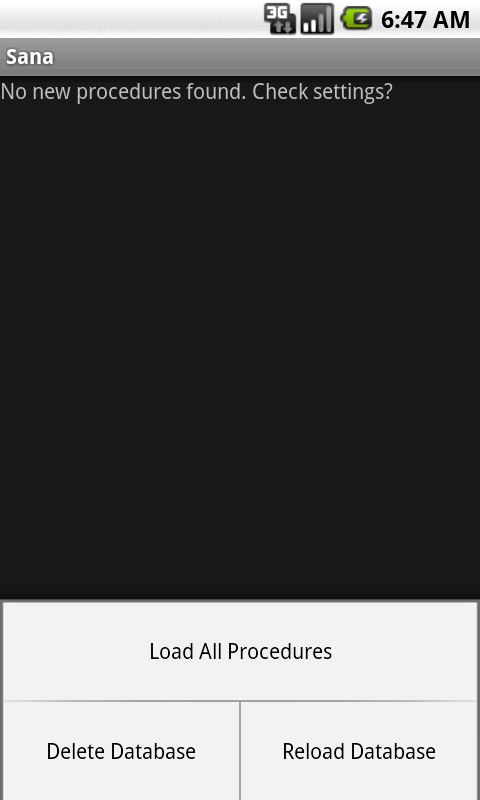
\includegraphics[scale=0.2,keepaspectratio=true]{client_settings_procedures_load.png}
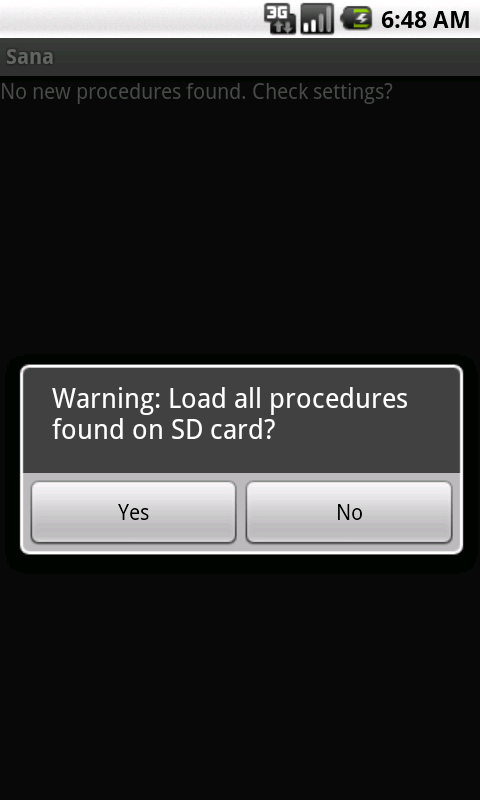
\includegraphics[scale=0.2,keepaspectratio=true]{client_settings_procedures_load_prompt.png}

\subsubsection{Viewing the results}
Clinical health workers in the field should now be able collect field data using
your new custom procedure and upload the results for review. Please see the
\textbf{Clinician Case Review} guide for full details regarding the review
process and user interface.
\clearpage{}

\cite{
http://www.nhlbi.nih.gov/guidelines/obesity/e_txtbk/txgd/algorthm/algorthm.htm}

\end{document}
